
\section{\trSymplectic{}\trManifold{}的例子}
\label{sec:examples-symplectic-manifolds}

显然，$\RR^n\times\RR^n$ 连同其常值\trForm{} $\sum dp_i\wedge dq_i$ 就是一个\trSymplectic{}\trManifold。

\textbf{\trCotangent{}丛}

设 $V$ 是一个\trManifold，我们来考虑其\trCotangent{}丛的全空间，投影为
\[
\pi\colon T^*V\longrightarrow V.
\]
在 $T^*V$ 上有一个\trCanonical{}的\trDifferential{} 1-\trForm{} $\lambda$，称为 \textbf{\trLiouville{}形式}（Liouville form），其定义为
\[
\lambda(x,\varphi)(X)=\varphi\bigl(T_{(x,\varphi)}\pi(X)\bigr)\text{，}
\]
其中 $x\in V$、$\varphi\in T^*_xV$ 且 $X\in T_{(x,\varphi)}(T^*V)$。很容易验证 $\omega=d\lambda$ 是\trNondegenerate{}的（更容易验证它是\trClosed{}的！）。若 $(q_1,\dotsc,q_n)$ 是 $V$ 的局部坐标，而 $(p_1,\dotsc,p_n)$ 是“对偶”坐标，则 $(p_1,\dotsc,p_n,q_1,\dotsc,q_n)$ 便是一个\trChart，在其中 $\lambda=\sum p_idq_i$ 并且 $\omega=\sum dp_i\wedge dq_i$。我们常说 $\omega$ 是\trCotangent{}丛上的“\trCanonical\trSymplecticForm”\footnote{这是\trExact{}\trSymplecticForm{}的又一个例子——显然是在非\trCompact{}的\trManifold{}上。}。上面给出的 $\RR^n\times\RR^n$ 的例子可以看成 $V=\RR^n$ 的情形。

\textbf{曲面}

在曲面 $W$ 上，\trDegree{}为 2 的\trDifferential\trForm{}全是\trClosed{}的。而且，在维数 2 的情形，说一个 2-\trForm{}是\trNondegenerate{}的，只不过是说它处处不为零。在曲面上，“\trSymplecticForm”的概念与“\trVolume{}形式”的概念重合：一切\trOrientable{}曲面都可以看作\trSymplectic{}\trManifold。

\begin{figure}[htbp]
\centering
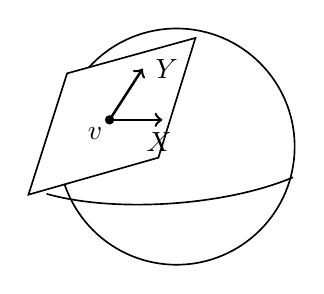
\begin{tikzpicture}[line width=0.6pt]
  \draw (0,0) circle (1.5);
  \draw (-1.65,-0.60) .. controls (-0.80,-0.84) and (0.60,-0.76) .. (1.48,-0.39);
  \draw[fill=white] (0.24,1.38) -- (-1.39,0.93) -- (-1.88,-0.61) -- (-0.23,-0.14) -- cycle;
  \fill (-0.85,0.34) circle (1.7pt);
  \node[below left=-1pt] at (-0.85,0.34) {$v$};
  \draw[->,line width=0.9pt] (-0.85,0.34) -- (-0.18,0.34);
  \node[below=1pt] at (-0.22,0.34) {$X$};
  \draw[->,line width=0.9pt] (-0.85,0.34) -- (-0.43,0.99);
  \node[right=1pt] at (-0.43,0.99) {$Y$};
\end{tikzpicture}
\caption{\trSphere{}上的\trSymplecticForm}
\label{fig:sphere-symplectic-form}
\end{figure}

\textbf{\trSphere}

我们考虑 $\RR^3$ 中的单位\trSphere{} $S^2$，它在一点 $v$ 处的\trTangentSpace{}就是与单位向量 $v$ \trOrthogonal{}的那个平面。我们令
\[
\omega_v(X,Y)=v\cdot(X\wedge Y)
\]
（\cref{fig:sphere-symplectic-form}）。这是一个\trNondegenerate{}的 2-\trForm{}（可以直接验证），因而是一个\trSymplecticForm。

\textbf{复\trProjectiveSpace}

要描述复\trProjectiveSpace{}上的\trSymplecticForm，最惬意的办法莫过于利用这个空间的商结构。于是让我们考虑
\[
\CC^{n+1}=\bigl\{p+iq\mid p\in\RR^{n+1},\ q\in\RR^{n+1}\bigr\}=\RR^{n+1}\times\RR^{n+1}\text{，}
\]
并赋予它 $\RR^{n+1}\times\RR^{n+1}$ 上通常的\trSymplecticForm。复\trProjectiveSpace{}就是商
\[
\CC^{n+1}-\{0\}\,/\,x\sim y\Longleftrightarrow\exists\lambda\neq 0\ \text{使得 }y=\lambda x\text{。}
\]
人们常常喜欢把它看成（\trCompact{}的）\trSphere{}的商：
\[
S^{2n+1}\,/\,x\sim y\Longleftrightarrow\exists\lambda\in S^1\ \text{使得 }y=\lambda x\text{，}
\]
比如说，要证它是一个（豪斯多夫而且）\trCompact{}的空间，这样看就很方便。于是我们有下面这张图表。
\[
\begin{tikzcd}[column sep=1.7cm,row sep=1.5cm]
S^{2n+1}\ar[r,"j"]\ar[d,"\pi"] & \CC^{n+1}-\{0\}\\
\CP^n(\CC) &
\end{tikzcd}
\]
2-\trForm{} $j^\star\omega$ 必然是\trDegenerate{}的。它在 $x\in S^{2n+1}$ 处的\trKernel{}是\trTangentSpace{} $T_xS^{2n+1}=x^\perp$ 中由向量 $ix$ 生成的直线（可以直接验证），于是 $(j^\star\omega)_x$ 便在商\trVectorSpace{} $T_xS^{2n+1}/ix$ 上诱导出一个\trNondegenerate{}的\trBilinearForm，而这个商\trVectorSpace{}不是别的，正是向量 $x$ 关于该\emph{\trHermitian{}}形式的\trOrthogonal{}空间。另一方面，由 $ix$ 生成的实直线也是
\[
T_x\pi\colon T_xS^{2n+1}\longrightarrow T_{\pi(x)}\CP^n(\CC)\text{，}
\]
的\trKernel，于是公式
\[
\sigma_{[x]}(Y,Z)=\omega_x(\widetilde{Y},\widetilde{Z})
\]
（其中 $x\in[x]$、$T_x\pi(\widetilde{Y})=Y$、$T_x\pi(\widetilde{Z})=Z$）的确定义了一个 2-\trForm，这样我们就证明了下面的结果。\footnote{译注：原书此处印作 “indeed defines a 2-form and that we have shown the following result”；“and that” 疑系赘笔（下文即该结果的陈述）；此处按文意径译。——译者注}

\begin{proposition}\label{thm:projective-symplectic-form}
在 $\CP^n(\CC)$ 上存在唯一的 2-\trForm{} $\sigma$ 满足
\[
\pi^\star\sigma=j^\star\omega\text{。}
\]
它是一个\trSymplecticForm。\noqed
\end{proposition}

\textbf{\trDarboux{}定理}

正如维数为 $2n$ 的\trSymplectic{}\trVectorSpace{}只有一种类型，局部地看，维数为 $2n$ 的\trSymplectic{}\trManifold{}也只有一种结构，这正是\trDarboux{}的那个著名定理所陈述的内容。

\begin{theorem}[\trDarboux]\label{thm:darboux-theorem}\BookIndexDefinition{T004}
设 $x$ 是\trSymplectic{}\trManifold{} $(W,\omega)$ 上的一点。存在以 $x$ 为中心的局部坐标 $(q_1,\dotsc,q_n,p_1,\dotsc,p_n)$，在其中
\[
\omega=\sum dp_i\wedge dq_i\text{。}
\]
\end{theorem}

只需去积分一个选取得当的\trVectorField{}就够了（循\trMoser{}的“路径”方法~[57]）……至于完整的证明，我们请读者去翻查他们心爱的任意一本辛几何教材，例如 [50] 或 [5]。
